\documentclass[12pt]{article}
\pagestyle{plain}

\usepackage[letterpaper,margin=1in]{geometry}
\usepackage{amsmath}
\usepackage[tone]{tipa}
\usepackage{amssymb}
\usepackage{array}
\usepackage{hyperref}
\usepackage{leipzig}
\usepackage{gb4e}
\noautomath
\usepackage{graphicx}
\graphicspath{ {./images/} }
\usepackage{wrapfig}
\usepackage{glossary-inline}
\usepackage{caption}

\makenoidxglossaries

\newleipzig{InessTwo}{iness2}{2d inessive}
\newleipzig{InessThree}{iness3}{3d inessive}
\newleipzig{AdessTwo}{adess2}{2d adessive}
\newleipzig{AdessThree}{adess3}{3d adessive}
\newleipzig{IllThree}{ill3}{3d illative}
\newleipzig{AllTwo}{all2}{2d allative}
\newleipzig{AllThree}{all3}{3d allative}
\newleipzig{AblThree}{abl3}{3d ablative}
\newleipzig{Ger}{ger}{gerund}
\newleipzig{Anim}{anim}{animate}
\newleipzig{Inanim}{inanim}{inanimate}
\newleipzig{Hst}{hst}{historical}
\newleipzig{Int}{int}{interrogative}
\newleipzig{Agt}{agt}{agentive}


\renewcommand{\L}{\textscl}

% Document
\begin{document}
    \title{A Reference Grammar of Psittacine}
    \date{}
    \author{Russell Emerine}

    \maketitle

    \newpage

    \tableofcontents

    \newpage


    \section{Background}\label{sec:background}
    Psittacine is a conlang set in the near future of the real world.
As they have done for millenia, humans continue to devastate the environment.
The rainforests continue shrinking and many animals are losing their habitat.
Under the threat of extinction,
parrots put their intelligence to use and create their own language,
and are using it to plot the downfall of humanity.

\begin{wrapfigure}{R}{0.46\textwidth}
    \caption{Alex performing a counting task.}
    \centering
    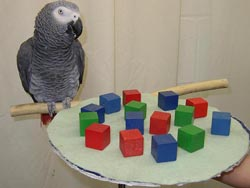
\includegraphics[scale=0.7]{alex}\label{fig:figure}
\end{wrapfigure}

Parrots are known to be some of the smartest non-human animals,
alongside great apes, dolphins, octopuses, elephants, and crows.
The possibility of parrots developing their own human-like language is not completely unreasonable.
Famously, many of them can imitate human language,
and a few
have claims to using and understanding human language.
Alex (\url{https://en.wikipedia.org/wiki/Alex_(parrot)}) was able to
perform remarkably complex tasks,
such as counting the number of objects with combinations of properties.
Alex also has been reported to be the only non-human animal to ever ask a question.

Parrots have very different physiology from humans,
but the sounds they will have in their language will be human-producible sounds.
Parrots can easily produce stops, fricatives, nasals, and a full range of vowels in a full range of phonations,
as well as many sounds humans cannot produce, such as chirps, beeps, and rapidly alternating tones.
I will only use sounds parrots and humans can both produce easily.
Since parrots don't have lips, their language will not have labial consonants or lip rounding.
(Alex reportedly had difficulty pronouncing ``paper''.)
The beak doesn't have teeth or an alveolar ridge,
but placing the tongue in approximately similar locations can make similar formant profiles.
The part of a parrot's brain responsible for cognition is the HVC,
originally purposed for processing and producing birdsong.
Since parrot language will have influence from birdsong,
it will be more reliant on tones than most human languages.

In the world of human expansion,
there are a number of different groups of parrots that
have unique interactions with humans and each other.
There are wild parrots from the rainforests who want to preserve their habitat,
and most of them want to destroy the humans.
There are feral urban parrots,
some who want to stop the humans and some who don't particularly care.
There are also domesticated parrots,
who mostly like humans (since those who don't run away).
The language has dialects that vary over the above groups, and by location.
Parrots and humans may learn each others' languages,
but have trouble producing certain sounds.

Parrots will also have their own writing system (not detailed in this book).
Some parrots may learn to use pens, but
the most natural way for parrots to write is to make scratches in bark using their beaks.
Parrots beaks have more strength and fine control than claws.
The writing system will consist mostly of short, straight strokes to reflect the medium of writing.

Parrots live all over the world, mostly in tropical areas.
Typical intelligent parrots live in natural hollows in tree canopies,
eat seeds, nuts, fruits, and occasionally bugs,
and are generally monogamous and nonterritorial.
Like humans, they are very social,
and their society could reasonably be organized similarly to that of humans.
In the story, they will develop government as they need high-level cooperation
to work against the humans.
They will also learn to use some technology.
Vocabulary and metaphors, including ones for the new technology,
will show influence from their social and dietary habits.


    \newpage


    \section{Phonology}\label{sec:phonology}
    \subsection{Consonants}\label{subsec:consonants}

Parrots do not have the same mouths as humans.
Also, parrots do not have a voice-producing larynx like humans do.
They instead produce sound at the syrinx,
an organ at the fork of the trachea found in birds.
While syrinxes are more powerful and flexible than larynxes,
the sounds they make are similar to human speech sounds for the purposes of notation.
So, sounds will be written as if they used standard human place and manner of articulation.

The biggest articulatory difference between humans and parrots is that
parrots don't have lips, so they are not able to produce labials.
In videos I found, experienced parrots can make labial-sounding sounds,
but they aren't created using the edge of the beak,
but by some other mechanism, perhaps the tongue.
Psittacine will not have labials at all.

Some other notable features I noticed in videos are that
parrots have very pronounced \textipa{[\:R]} and \textipa{[l]} sounds,
and don't make human-like trills.
I chose to expand on the sound of strong approximants by including more approximants.
I chose for there to only be voiceless plosives and fricatives,
to produce a more ``chitter-chatter'' kind of sound.

\begin{center}
    \begin{tabular}{|c|c|c|c|c|}
        \hline
        & Alveolar
        & Retroflex
        & Velar
        & Glottal \\
        \hline
        Plosive
        & \textipa{/t/} t
        &
        & \textipa{/k/} k
        & \\
        \hline
        Nasal
        & \textipa{/n/} n
        &
        & \textipa{/N/} g
        & \\
        \hline
        Fricative
        & \textipa{/s/} s
        & \textipa{/\:s/} x
        &
        & \textipa{/h/} h \\
        \hline
        Affricate
        & \textipa{/\t{ts}/} z
        & \textipa{/\t{t\:s}/} c
        &
        & \\
        \hline
        Approximant
        &
        & \textipa{/\:R/} r
        & \textipa{/w/} w
        & \\
        \hline
        Lateral Approximant
        & \textipa{/l/} l
        &
        & \textipa{/\L/} ł
        & \\
        \hline
    \end{tabular}
\end{center}

\subsection{Vowels}\label{subsec:vowels}

Parrots have a complete range of vowel qualities,
with no significant difference from humans.
While they don't have lips, they can make rounded vowels with no problems,
possibly using their tongue.
I chose the following inventory because just because it contains both
\textipa{/\ae/} and \textipa{/A/},
which I plan to use in specific vocabulary items,
and it isn't too imbalanced.

\begin{center}
    \begin{tabular}{|c|c|c|c|}
        \hline
        & Front             & Mid             & Back            \\
        \hline
        High & \textipa{/i/} i   & \textipa{/1/} y & \textipa{/u/} u \\
        \hline
        Mid  & \textipa{/e/} e   &                 &                 \\
        \hline
        Low  & \textipa{/\ae/} a &                 & \textipa{/A/} o \\
        \hline
    \end{tabular}
\end{center}

There are no diphthongs.
There are some instances of adjacent vowels,
all pronounced in hiatus.

\subsection{Tones and Phonation}\label{subsec:tones-and-phonation}

Since parrot speech is similar to birdsong,
Psittacine will have a relatively high number of tones.
Parrots also have atypical phonation.
Creaky voice seems to be especially common in the videos I saw.
(Interestly, the combination of tone contours and phonation is also present in Vietnamese.)

Tones will only be applied to approximately one syllable per content morpheme,
in a manner similar to the toned pitch accent system in Norwegian and Swedish.
The tones on the accented syllables may allophonically affect tone in surrounding syllables,
i.e.\ a low tone start on an accented syllable may make the syllable before also low.

The following tones and phonations will be available on all vowels.
They are demonstrated on \textipa{/A/}.

\begin{center}
    \begin{tabular}{|c|c|}
        \hline
        Description   & Transcription               \\
        \hline
        Mid tone      & \textipa{/A\tone{22}/} o    \\
        \hline
        High tone     & \textipa{/A\tone{55}/} ō    \\
        \hline
        Rising tone   & \textipa{/A\tone{35}/} ó    \\
        \hline
        Falling tone  & \textipa{/A\tone{51}/} ò    \\
        \hline
        Peaking tone  & \textipa{/A\tone{352}/} ô   \\
        \hline
        Creaky low    & \textipa{/\~*A\tone{11}/} õ \\
        \hline
        Creaky rising & \textipa{/\~*A\tone{13}/} ǒ \\
        \hline
    \end{tabular}
\end{center}

\subsection{Phonotactics}\label{subsec:phonotactics}

The syllable structure of the language is (C)(R)V(C),
where C is a consonant, R is a (possibly lateral) approximant, and V is a vowel,
with some tone if it is accented.
When there is a syllable-initial consonant cluster,
only the following CR groups are possible, chosen based on ease of pronunciation:
\begin{center}
    \begin{tabular}{|c|c|c|c|c|c|c|c|c|c|}
        \hline
        & t          & k          & n          & g          & s          & x          & h          & z          & c          \\
        \hline
        r &            & \checkmark &            & \checkmark &            & \checkmark & \checkmark &            & \checkmark \\
        \hline
        w & \checkmark & \checkmark & \checkmark & \checkmark & \checkmark & \checkmark & \checkmark & \checkmark & \checkmark \\
        \hline
        l &            & \checkmark &            &            & \checkmark & \checkmark & \checkmark &            &            \\
        \hline
        ł &            & \checkmark &            &            & \checkmark & \checkmark & \checkmark &            &            \\
        \hline
    \end{tabular}
\end{center}

Otherwise, any consonant can start a syllable.

Any consonant other than h can end a syllable.

The central vowel is intended to be just one vowel, not a diphthong.

\subsection{Example Phonotactically Sound Words}\label{subsec:example-phonotactically-sound-words}
\begin{itemize}
    \item wùg \textipa{/wuN\tone{51}/} ``me''
    \item słygiz \textipa{/s\L{}1Ni\t{ts}\tone{33}/} ``vine''
    \item hengó \textipa{/henNA\tone{35}/} ``forest''
    \item rõk \textipa{/\:R\~*Ak\tone{11}/} ``mountain''
    \item kłas \textipa{/k\L{}\~*\ae{}s\tone{13}/} ``glass''
\end{itemize}
    \newpage


    \section{Pronouns}\label{sec:pronouns}
    \subsection{Pronouns}\label{subsec:pronouns}

Pronouns pluralize by reduplication,
and have an animacy distinction in 3rd person pronouns.
Mass nouns are considered singular.
First person plural can be inclusive or exclusive.
Animals are animate, and everything else is inanimate.
The decision to have pluralization for pronouns
but not for nouns is taken from Chinese.

There is a 4th person ``generic'' pronoun,
with singular used for generic ``you'' or generic ``one''
and plural used for generic ``they''.
There is a single reflexive pronoun
that applies for any person.
It is pluralized to match its antecedent.

There are proximal and distal demonstratives
in animate and inanimate forms.
These are listed as pronouns.
The adjective forms, e.g.\ ``this book'', are just normal adjectives,
which will be derived from the pronoun forms with -hły attached.
The adjective forms do not have plurals.

\begin{center}
    \begin{tabular}{|c|c|c|}
        \hline
        Person                                  & Singular & Plural   \\
        \hline
        1st                                     & wùg      & wùgwùg   \\
        \hline
        2nd                                     & à        & àà       \\
        \hline
        3rd animate                             & gó       & gógó     \\
        \hline
        3rd inanimate                           & zine     & zinezine \\
        \hline
        4th                                     & kȳt      & kȳtkȳt   \\
        \hline
        Reflexive (self)                        & xeł      & xełxeł   \\
        \hline
        Proximal demonstrative animate (this)   & nôr      & nôrnôr   \\
        \hline
        Proximal demonstrative inanimate (this) & slôr     & slôrslôr \\
        \hline
        Distal demonstrative animate (that)     & kũx      & kũxkũx   \\
        \hline
        Distal demonstrative inanimate (that)   & krũx     & krũxkrũx \\
        \hline
    \end{tabular}
\end{center}

\subsection{Examples}\label{subsec:examples}

The following are a few examples of pronoun usage
that are less obvious.

\begin{exe}
    \ex
    \glt
    kȳt xwéty gòni
    \glll
    kȳt xwé=ty gòn=i \\
    4\Sg{} knowledge=\Poss{} faith=\IllThree{} \\
    one knowledge=\Poss{} faith=into \\
    \glt
    faith in one's knowledge
\end{exe}
An instance of a 4th person singular pronoun in use.

\begin{exe}
    \ex
    xrôł kȳtkȳt kazcǒ gó gón
    \glll
    xrôł kȳtkȳt kazcǒ gó gón \\
    say 4\Pl{} want 3\Sg{}.\Anim{} food \\
    say them want him food \\
    \glt
    They say he wants food.
\end{exe}
An instance of a 4th person plural pronoun in use.
The English phrase ``They say \dots'' is the most typical
kind of usage for 4th person plural.

\begin{exe}
    \ex
    \glll
    xeł krârwik=ty  \\
    \Refl{}.\Sg{} idea=\Poss{} \\
    self idea=\Poss{} \\
    \glt
    one's own idea
\end{exe}
An example of a reflexive pronoun in use.
Without an antecedent, this could mean
``my own idea'',
``your own idea'',
``its own idea'',
or
``one's own idea''.
Reflexive possessives don't translate into English perfectly,
so as an example,
it would be used in
``He disliked his idea'',
where ``his'' refers to the subject rather than someone else.


    \newpage


    \section{Nouns and Stance Forms}\label{sec:nouns-and-stance-forms}
    Inflectional morphology in nouns is very simple.
Definiteness, gender, number, and case are not marked.

Stance forms are the main form of inflectional morphology for nouns.
They are used instead of adpositions,
and have a unique mechanism that I am not aware of in any natural language.

\subsection{Inspiration for Stance Forms}\label{subsec:inspiration-for-stance-forms}

While browsing Wikipedia at one point,
I learned that some languages, most notably in the Semitic branch,
have a ``construct state''
which involves modifying a noun to indicate
that it is possessed by another noun.
In Arabic, this process is called \textit{iḍāfah}.
One example Wikipedia gives in Egyptian Arabic is
\begin{center}
    \begin{tabular}{|c|c|}
        \hline
        malika    & a queen              \\
        \hline
        il-malika & the queen            \\
        \hline
        malik(i)t & a/the queen of \dots \\
        \hline
    \end{tabular}
\end{center}
((i) is present or absent according to sandhi.)

I found this translation with ``of \dots'' unusual
and decided it would be interesting to generalize this to
positional as well as possessive relationships.
When relating some noun (or noun phrase) to some location (or possessor),
rather than keeping the noun the same
and attaching an adposition to the location,
I will modify the noun and keep the location the same.
As far as I'm aware, no natural language does this,
so I get to invent terminology!
I call the modification of the noun a ``stance form'',
since it indicates how the noun is positioned,
which is a ``stance'' in a sense.

\subsection{Inspirational for Dimensional Distinction}\label{subsec:inspirational-for-dimensional-distinction}

I also decided that since birds can fly,
they live more three-dimensional lives than humans.
Then, it is plausible that they would have
more nuanced positional relations than humans,
including a distinction between three-dimensional ``in'' and ``on''
and two-dimensional ``in'' and ``on''.
For example,
there may be walnuts three-dimensionally in a loaf of banana bread,
while Rome is two-dimensionally in Italy (as on a map).

One source of inspiration for this is that in middle school,
I got a 3D chess variant called YAVOCH\@.
The lore in YAVOCH is that aliens are confronting humans
and have given humans spaceships to allow a fair fight.
Humans were unable to pilot the spaceships until
they connected animal brain patterns to the systems.
In particular, the animal brains (including birds)
were better with 3D spatial movement than human logic was.

There was also a time in a math class long ago when the teacher
referenced a point ``on'' a circle, meaning on the outline,
but many students assumed it was an interior point.
I thought it would be interesting to have a distinction.

\subsection{Usage of Stance Forms}\label{subsec:usage-of-stance-forms}

Stance forms will cover the following semantic roles,
with corresponding English forms:
\begin{itemize}
    \item
    Location of being
    \begin{itemize}
        \item 2D in, 2D on, 3D in, 3D on
        \item over, under, near, far from
    \end{itemize}
    \item
    Location of motion, as origin, destination, or path
    \begin{itemize}
        \item 2D into, onto, out of, off of, through, across, and 3D \dots
        \item towards, away from
    \end{itemize}
    \item
    Possession
\end{itemize}

Stance forms can also be used with partial nouns,
like ``top'' or ``side'',
which each are connected to their own nouns as possessed forms.
The same partial noun can take on different meanings according to 2D or 3D interpretation.
This can lead to very detailed descriptions of position or movement,
such as going up a mountain to reach its top face (2D ``top''),
vs.\ going up a mountain to fly in the space at its peak (3D ``top'').

Using a stance form without a verb will translate to
locational ``be'', ``go'', or possession,
according to the meaning of the stance form.
This can be thought of as a form of null copula.

The specific morphology of stance forms will be a simple suffix clitic.
The syntax is that the location (or possessor) will come first,
and the noun with the stance form will come second.

\newpage

\subsection{Examples}\label{subsec:examples2}

\begin{exe}
    \ex
    \glt
    hlātu gòna
    \glll
    hlātu gò=na \\
    plate fruit=\AdessTwo{} \\
    plate fruit=on \\
    \glt
    The fruit is on (2D) the plate.
\end{exe}

\begin{figure}[ht]
    \caption*{(4) Considering the plate as a two-dimensional region, the fruit is on the edge.}
    \centering
    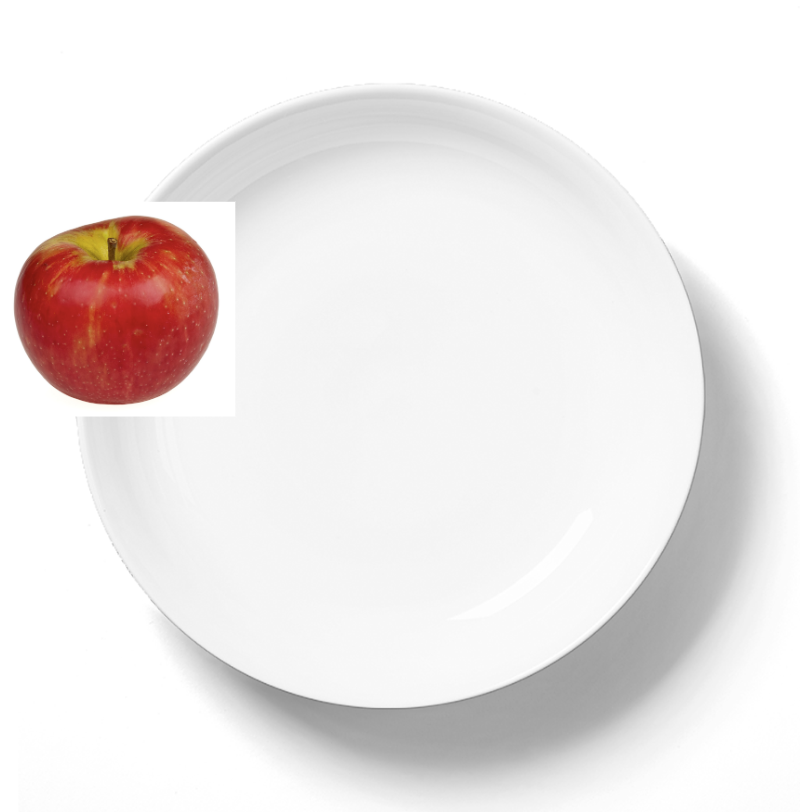
\includegraphics[scale=0.3]{adess2}\label{fig:figure2}
\end{figure}

\begin{exe}
    \ex
    \glt
    hlātu gòni
    \glll
    hlātu gò=ni \\
    plate fruit=\InessTwo{} \\
    plate fruit=in \\
    \glt
    The fruit is in (2D) the plate.
\end{exe}

\begin{figure}[ht]
    \caption*{(5) Considering the plate as a two-dimensional region, the fruit is in the interior.}
    \centering
    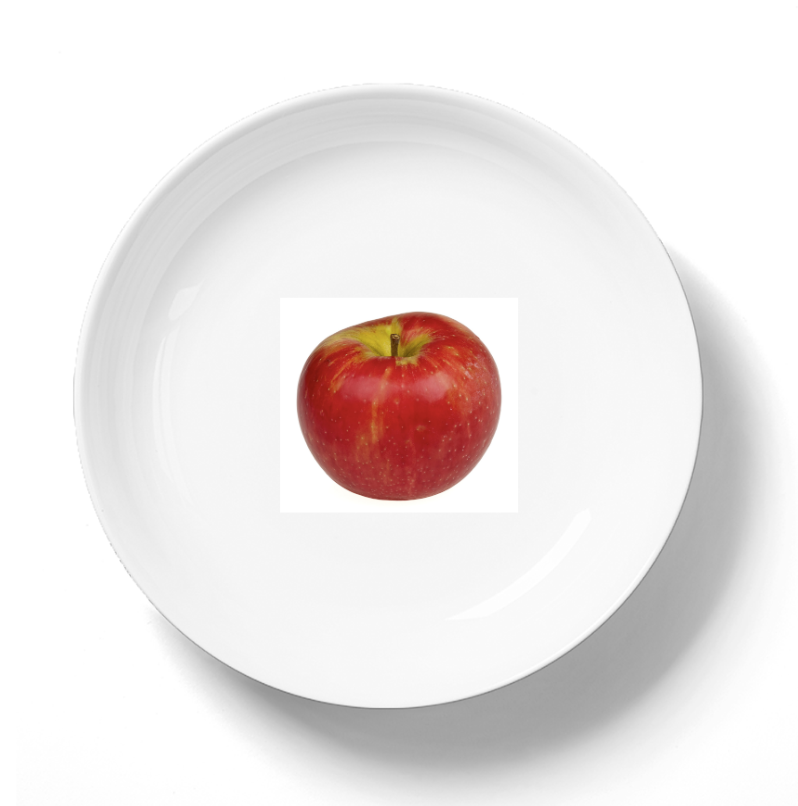
\includegraphics[scale=0.3]{iness2}\label{fig:figure3}
\end{figure}

\newpage

\begin{exe}
    \ex
    \glt
    hlātu gòla
    \glll
    hlātu gò=la \\
    plate fruit=\AdessThree{} \\
    plate fruit=on \\
    \glt
    The fruit is on (3D) the plate.
\end{exe}

\begin{figure}[ht]
    \caption*{(6) Considering the plate as a three-dimensional object, the fruit is at the exterior.}
    \centering
    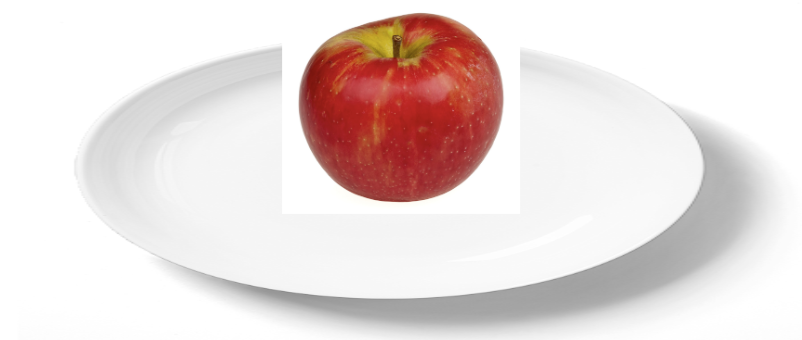
\includegraphics[scale=0.3]{adess3.1}\label{fig:figure4}
\end{figure}

\begin{figure}[ht]
    \caption*{(6) Again considering the plate as a three-dimensional object, the fruit is painted onto the exterior.}
    \centering
    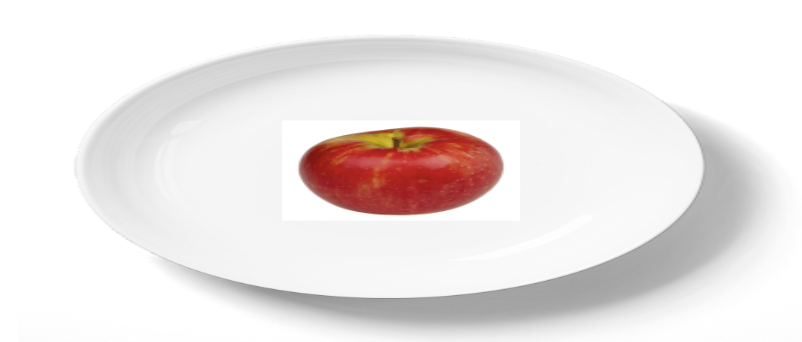
\includegraphics[scale=0.3]{adess3.2}\label{fig:figure5}
\end{figure}

\begin{exe}
    \ex
    \glt
    hlātu gòli
    \glll
    hlātu gò=li \\
    plate fruit=\InessThree{} \\
    plate fruit=in \\
    \glt
    The fruit is in (3D) the plate.
\end{exe}

\begin{figure}[ht]
    \caption*{(7) Considering the plate as a three-dimensional object, the fruit in the interior, surrounded by ceramic.}
    \centering
    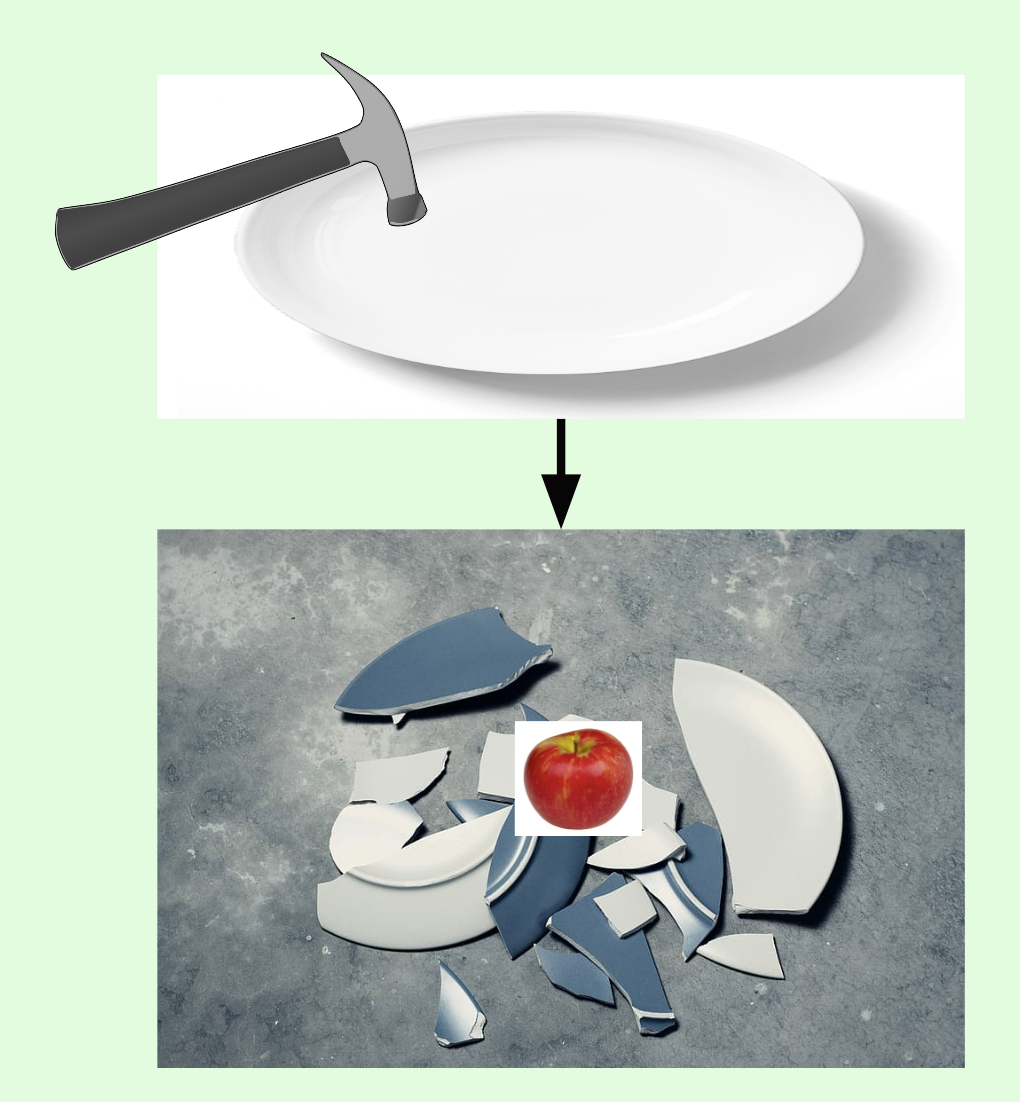
\includegraphics[scale=0.27]{iness3}\label{fig:figure6}
\end{figure}

\newpage

\begin{exe}
    \ex
    \glll
    hengó wùg=ni \\
    forest 1\Sg{}=\InessTwo{}\\
    forest I=in \\
    \glt
    I am in the forest.
\end{exe}

Large areas like forests and countries are considered two-dimensional
since they cover a flat area of the earth.

\begin{exe}
    \ex
    \glll
    rõk kwałŷx=la wùg lelō=ty=li \\
    mountain tree=\AdessThree{} 1\Sg{} nest=\Poss{}=\InessThree{} \\
    mountain tree=on I nest=\Poss{}=in \\
    \glt
    My nest is in the tree on the mountain.
\end{exe}

Trees and mountains are considered three-dimensional.
Nestled stance phrases behave as expected.
Here, ``nest'' is part of two stance phrases,
one of possession and one of location.
The stance suffixes are placed one after the other,
and the corresponding nouns are determined by order and context.

\begin{exe}
    \ex
    \glll
    kwałŷx xâr=ty słygiz=la \\
    tree top=\Poss{} vine=\AdessThree{} \\
    tree top=\Poss{} vine=towards \\
    \glt
    The vine goes up the tree.
    \ex
    \glll
    crizǐ xâr=ty słygiz=na \\
    house top=\Poss{} vine=\AdessTwo{} \\
    house top=\Poss{} vine=towards \\
    \glt
    The vine goes up the house.
\end{exe}

When a vine goes up a tree,
it grows outwards in the space near the top of the tree,
spreading in all directions.
When a vine goes up a house,
it lays flat on the roof,
restricted to the plane the roof is in.
So, ``top'' is used as 3D for the example with the tree,
and as 2D for the example with the house.


    \newpage


    \section{Adjectives}\label{sec:adjectives}
    Adjectives are very simple.
They are simply placed before the noun.

\subsection{Adjectivization}\label{subsec:adjectivization}
The -hły suffix marks adjectivization.
The most important use of -hły is be turning material nouns into adjectives.
As shown in the section about pronouns,
-hły is also used to turn demonstrative pronouns into demonstrative determiners,
which also act as normal adjectives.

\begin{exe}
    \ex
    \glt
    xrõk gón slôrhły hlātula
    \glll
    xrõk gón slôr-hły hlātu=la \\
    amazing food \Dem{}.\Prox{}-\Adj{} plate=\AdessThree{} \\
    amazing food this plate=on \\
    \glt
    the amazing food on this plate
\end{exe}
This example is ambiguous;
the above phrase also could mean
``the amazing food on the plate made of this [material]''.

\begin{exe}
    \ex
    \glt
    twazwahły wihǔ
    \glll
    twazwa-hły wihǔ \\
    metal-\Adj{} bird \\
    metal bird \\
    \glt
    airplane
    \ex
    \glt
    kłǎshły nūr
    \glll
    kłǎs-hły nūr \\
    glass-\Adj{} light \\
    glass light \\
    \glt
    lightbulb
\end{exe}

A number of terms that may be simple or compound words in English
are referred to with adjective-noun phrases in Psittacine.
Material adjectives are common for this.

\subsection{Adverbs}\label{subsec:adverbs}

Adverbs are just adjectives placed before verbs rather than before nouns.

\begin{exe}
    \ex
    \glt
    cỳłty kwǒn wùg.
    \glll
    cỳłty kwǒn wùg \\
    happy sleep 1\Sg{} \\
    happy sleep me \\
    \glt
    I sleep happily.
\end{exe}


    \newpage


    \section{Verbs}\label{sec:verbs}
    Verbs in Psittacine are rather simple morphologically.
They have some inflectional morphology but
do not change for agreement in person or number with the subject or object.
However, they do have more complicated syntactic mechanisms.

\subsection{Word Order}\label{subsec:word-order}

The typical word order is
\begin{center}
    \quad Verb \quad Subject \quad [\quad Direct Object \quad  [ \quad Indirect Object \quad ] \quad ]
\end{center}
where each verb takes a specific number of arguments.
The language is strictly nominative-accusative.
Word order is the only indication of which noun is the subject, direct object, or indirect object.

\begin{exe}
    \ex
    \glt
    kwǒn wihǔ.
    \glll
    kwǒn wihǔ \\
    sleep bird \\
    sleep bird \\
    \glt
    The bird sleeps.
\end{exe}

\begin{exe}
    \ex
    \glt
    krân wùg wug.
    \glll
    krân wùg wug \\
    see 1\Sg{} dog \\
    see me dog \\
    \glt
    I see the dog.
\end{exe}

\begin{exe}
    \ex
    \glt
    krân wug wùg.
    \glll
    krân wug wùg \\
    see dog 1\Sg{} \\
    see dog me \\
    \glt
    The dog sees me.
\end{exe}

\begin{exe}
    \ex
    \glt
    gāw gó hlātu wùg.
    \glll
    gāw gó hlātu wùg \\
    give 3\Sg{}.\Anim{} plate 1\Sg{} \\
    give him plate me \\
    \glt
    He gives me a plate.
\end{exe}

\subsection{Auxiliary Verbs}\label{subsec:auxiliary-verbs}

Verbs have an intrinsic valency.
Some are intransitive, some are transitive, and a few are ditransitive.
The language uses auxiliary verbs with gerunds to change transitivity.

Gerunds are formed by adding the suffix \textit{-ga} to a verb.

The auxiliary verb \textit{zà} ``do''
can take a transitive or ditransitive gerund as an object
and produce an intransitive form.
\textit{zà} is used exclusively for changing valency
and cannot be used for sentences like ``I do the homework''.

\begin{exe}
    \ex
    \glt
    zà wihǔ kōgga.
    \glll
    zà wihǔ kōg-ga \\
    do bird eat-\Ger{} \\
    do bird eating \\
    \glt
    The bird eats.
\end{exe}

\begin{exe}
    \ex
    \glt
    zà kwałŷx gāwga.
    \glll
    zà kwałŷx gāw-ga \\
    do tree give-\Ger{} \\
    do tree giving \\
    \glt
    The tree gives.
    /
    The tree provides.
\end{exe}

The auxiliary verb \textit{hłĩk} ``make, cause''
can take a gerund as an object.
If the gerund is possessed by a noun,
the noun is the patient of the sentence.
The causative formed is the most general type of causative,
where the patient is not necessarily forced.

In the following two examples,
\textit{xrîz} is naturally intransitive.

\begin{exe}
    \ex
    \glt
    hłĩk howeg kwałŷx xrîzgaty.
    \glll
    hłĩk howeg kwałŷx xrîz-ga=ty \\
    make wind tree shake-\Ger{}=\Poss{} \\
    make wind tree shaking=\Poss{} \\
    \glt
    The wind makes the tree shake.
    /
    The wind shakes the tree.
    \ex
    \glt
    hłĩk howeg xrîzga.
    \glll
    hłĩk howeg xrîz-ga \\
    make wind shake-\Ger{} \\
    make wind shaking \\
    \glt
    The wind shakes [things].
    \ex
    \glt
    hłîk wihǔ xǎw wihǔ kōggaty.
    \glll
    hłîk wihǔ xǎw wihǔ kōg-ga=ty \\
    make bird small bird eat-\Ger{}=\Poss{} \\
    make bird small bird eating=\Poss{} \\
    \glt
    The bird makes the chick eat.
    /
    The bird feeds the chick.
\end{exe}

The auxiliary verb \textit{xal} ``make, cause'',
similarly to \textit{hłĩk},
takes a gerund as an object.
However, \textit{xal} also takes in indirect object,
which acts as the direct object of the original transitive verb.

\begin{exe}
    \ex
    \glt
    xal wihǔ xǎw wihǔ kōggaty gò.
    \glll
    xal wihǔ xǎw wihǔ kōg-ga=ty gò \\
    make bird small bird eat-\Ger{}=\Poss{} fruit \\
    make bird small bird eating=\Poss{} fruit \\
    \glt
    The bird makes the chick eat fruit.
    /
    The bird feeds the chick fruit.
\end{exe}

\subsection{Replacements for be, have, and go}\label{subsec:replacements-for-be-have-and-go}

The language uses the zero copula.
This may be used to relate two nouns
or state a noun in a stance form.
Because of the language's complex directional system,
this takes the place of ``to be'', ``to go'', and ``to have''.

\begin{exe}
    \ex
    \glt
    wùg hełǎ.
    \glll
    wùg hełǎ \\
    1\Sg{} human \\
    me human \\
    \glt
    I am a human.
\end{exe}

\begin{exe}
    \ex
    \glt
    zine wùg zyla nũrty.
    \glll
    zine wùg zyla nũr=ty \\
    3\Sg{}.\Inanim{} 1\Sg{} blue feather=\Poss{} \\
    it me blue feather=\Poss{} \\
    \glt
    It's my blue feather.
\end{exe}

\begin{exe}
    \ex
    \glt
    wùg zyla nũrty.
    \glll
    wùg zyla nũr=ty \\
    1\Sg{} blue feather=\Poss{} \\
    me blue feather=\Poss{} \\
    \glt
    The blue feather is mine.
    /
    I have a blue feather.
\end{exe}

\begin{exe}
    \ex
    \glt
    crizǐ xârty słygizna.
    \glll
    crizǐ xâr=ty słygiz=na \\
    house top=\Poss{} vine=\AdessTwo{} \\
    house top=\Poss{} vine=towards \\
    \glt
    The vine goes up the house.
\end{exe}

Statement of existence equivalent to ``there is''
does not have a unique construction.
Rather, it is treated as a place having things.
If the statement of existence is too general
to be tied to a particular place,
``here'' is used by default,
or if that is ambiguous,
``the world'' is used.

\begin{exe}
    \ex
    \glt
    kwałŷx gòty.
    \glll
    kwałŷx gò=ty \\
    tree fruit=\Poss{} \\
    tree fruit=\Poss{} \\
    \glt
    The tree has fruit.
    /
    There is fruit in the tree.
\end{exe}

\begin{exe}
    \ex
    \glt
    kûk crizǐty.
    \glll
    kûk crizǐ=ty \\
    here house=\Poss{} \\
    here house=\Poss{} \\
    \glt
    There are houses here.
    /
    There are houses [in general].
\end{exe}

Adjectives act like intransitive verbs.

\begin{exe}
    \ex
    \glt
    zyla nũr.
    \glll
    zyla nũr \\
    blue feather \\
    blue feather \\
    \glt
    The feather is blue.
\end{exe}

\subsection{Negation}\label{subsec:negation}
A verb is negated by adding the suffix \textit{-hy}.

\begin{exe}
    \ex
    \glt
    lȳthy èt húgni.
    \glll
    lȳt-hy èt húg=ni \\
    fly-\Neg{} night bees=\InessTwo{} \\
    fly-not night bees=at \\
    \glt
    The bees do not fly at night.
\end{exe}

\begin{exe}
    \ex
    \glt
    kōghy wùg rãw.
    \glll
    kōg-hy wùg rãw \\
    eat-\Neg{} 1\Sg{} meat \\
    eat-not me meat \\
    \glt
    I do not eat meat.
\end{exe}

Since adjectives are like verbs, the suffix can be added directly to an adjective.

\begin{exe}
    \ex
    \glt
    zine twazwahłyhy.
    \glll
    zine twazwa-hły-hy \\
    3\Sg{}.\Inanim{} metal-\Adj{}-\Neg{} \\
    it metal-not \\
    \glt
    It's not made of metal.
\end{exe}

This also applies to adjectives that are not directly acting as verbs.
The most obvious application of this is in disambiguation,
but it can also just be a simple description (not quite an antonym, just a lack of a trait).
\begin{exe}
    \ex
    \glt
    kōghy wihǔ zighy gò.
    \glll
    kōg-hy wihǔ zig-hy gò \\
    eat-\Neg{} bird fresh-\Neg{} fruit \\
    eat-not bird fresh-not fruit \\
    \glt
    The birds do not eat unfresh fruit.
\end{exe}

Since there is no verb when relating two nouns
or stating a noun in a stance form,
a special verb must be used for negating such a statement.
\textit{ì} ``be / go'' is used
with the negation suffix attached.
\textit{ì} is special in that
it is neither transitive nor intransitive,
and accepts either two nouns or one noun in a stance form.

\begin{exe}
    \ex
    \glt
    ìhy wùg wihǔ.
    \glll
    ì-hy wùg wihǔ \\
    be-\Neg{} 1\Sg{} bird \\
    be-not me bird \\
    \glt
    I am not a bird.
\end{exe}

\begin{exe}
    \ex
    \glt
    ìhy èt kûkni twazwahły hūtna.
    \glll
    ì-hy èt kûk=ni twazwa-hły hūt=na \\
    be-\Neg{} night here=\InessTwo{} metal-\Adj{} caterpillar=\AdessTwo{} \\
    be-not night here=at metal caterpillar=towards \\
    \glt
    The trains do not go here at night.
\end{exe}

\subsection{Tense}\label{subsec:tense}
There are four tenses, present, past, future, and remote past,
used for example when telling stories.
The present is unmarked.
The other tenses are indicated by verbal suffixes.

\begin{exe}
    \ex
    \glt
    kwǒnce wùg.
    \glll
    kwǒn-ce wùg \\
    sleep-\Pst{} 1\Sg{} \\
    slept me \\
    \glt
    I slept.
\end{exe}

\begin{exe}
    \ex
    \glt
    zàcat takís gréga.
    \glll
    zà-cat takís gré-ga \\
    do-\Hst{} country farm-\Ger{} \\
    did country farming \\
    \glt
    The country farmed [once upon a time].
\end{exe}



The tense suffixes occur before \textit{-hy}.
\begin{exe}
    \ex
    \glt
    xwèwykhy wùg agìty zine.
    \glll
    xwè-wyk-hy wùg agì=ty zine \\
    know-\Fut{}-\Neg{} 1\Sg{} friend=\Poss{} 3\Sg{}.\Inanim{} \\
    know-will-not me friend=\Poss{} it \\
    \glt
    My friend will not know it.
\end{exe}

``be'', ``have'', and ``go''
are usually expressed without a verb in the present tense.
In the other tenses, they must have a verb.
Forms which take one noun in a stance form use the same \textit{ì}
that negation uses.
However, forms which relate two nouns
use the suppletive verb \textit{sèt}, which is not used in present tense.

\begin{exe}
    \ex
    \glt
    sètwyk hełǎ wùg agìty.
    \glll
    sèt-wyk hełǎ wùg agì=ty \\
    be-\Fut{} human 1\Sg{} friend=\Poss{} \\
    be-will human me friend=\Poss{} \\
    \glt
    The human will be my friend.
\end{exe}

\begin{exe}
    \ex
    \glt
    ìce lutlùt wùgna.
    \glll
    ì-ce lutlùt wùg=na \\
    be-\Pst{} river 1\Sg{}=\AdessTwo{} \\
    was river me=at \\
    \glt
    I was at the river.
\end{exe}

\begin{exe}
    \ex
    \glt
    ìce lutlùt wùgza.
    \glll
    ì-ce lutlùt wùg=za \\
    be-\Pst{} river 1\Sg{}=\AllTwo{} \\
    went river me=to \\
    \glt
    I went to the river.
\end{exe}

\begin{exe}
    \ex
    \glt
    ìcat à gónty.
    \glll
    ì-cat à gón=ty \\
    be-\Fut{} 2\Sg{} food=\Poss{} \\
    have-will you food=\Poss{} \\
    \glt
    The food will be yours.
    /
    You will have food.
\end{exe}

Adjectives simply take tense suffixes like normal verbs.

\begin{exe}
    \ex
    \glt
    xǎwcat wùgwùg.
    \glll
    xǎw-cat wùgwùg \\
    young-\Hst{} 1\Pl{} \\
    young-were we \\
    \glt
    We were young [long ago, or in a story].
\end{exe}

\subsection{Aspect and Mood}\label{subsec:aspect-and-mood}
Semantic aspect and mood are not indicated grammatically.
Rather, if they have reason to be expressed, they are just adverbs
(or sometimes complex constructions if more detail is required).

Example for progressive aspect.
\begin{exe}
    \ex
    \glt
    taktak lȳtce wihǔ.
    \glll
    taktak lȳt-ce wihǔ \\
    for.some.time fly-\Pst{} bird \\
    for.some.time flew bird \\
    \glt
    The bird flew for some time.
    /
    The bird was flying.
\end{exe}

Example for iterative aspect.
\begin{exe}
    \ex
    \glt
    ò xenãtce wùg sōkrohły lâl.
    \glll
    ò xenãt-ce wùg sōkro-hły lâl \\
    again read-\Pst{} 1\Sg{} leaf-\Adj{} song \\
    again read me leafy song \\
    \glt
    I read the book again.
    /
    I reread the book.
\end{exe}

Example for potential mood.
Most adverbs don't apply to the copula in a natural way,
but this is an instance where it can happen.
Adverbs applied to the null copula just end up at the start of the sentence.
\begin{exe}
    \ex
    \glt
    cēłta zine rõk.
    \glll
    cēłta zine rõk \\
    might 3\Sg{}.\Inanim{} mountain \\
    might it mountain \\
    \glt
    It might be the mountain.
\end{exe}


    \newpage


    \section{Syntax}\label{sec:syntax}
    Basic word order has already been explained.
Once again, it is
\begin{center}
    \quad Verb \quad Subject \quad [\quad Direct Object \quad  [ \quad Indirect Object \quad ] \quad ]
\end{center}
There are a number of other syntactic mechanisms for more structurally complex sentences.

\subsection{Conjunctions and Conditionals}\label{subsec:conjunctions-and-conditionals}

The basic conjunctions are \textit{tot} ``and''
and \textit{cec} ``or''.
When joining two items, the conjunction is placed between.
When joining three or more items,
the conjunction may be placed between each item
or may be used just once after all the items.
Parallel items all undergo any expected inflection.

\begin{exe}
    \ex
    \glt
    cǎwce nī tot wihǔ.
    \glll
    cǎw-ce nī tot wihǔ \\
    loud-\Pst{} cat and bird \\
    loud-were cat and bird \\
    \glt
    The cat and the bird were loud.
\end{exe}

(\textit{kȳhi} is an adverb.)
\begin{exe}
    \ex
    \glt
    kȳhi à húgty hūtty crákty cec.
    \glll
    kȳhi à húg=ty hūt=ty crák=ty cec \\
    able 2\Sg{} bee=\Poss{} caterpillar=\Poss{} ant=\Poss{} or \\
    able you bee=\Poss{} caterpillar=\Poss{} ant=\Poss{} or \\
    \glt
    You can have the bee, the caterpillar, or the ant.
\end{exe}

\begin{exe}
    \ex
    \glt
    lȳtce, toktõkce, slêxce tot wùgwùg.
    \glll
    lȳt-ce toktõk-ce slêx-ce tot wùgwùg \\
    fly-\Pst{} run-\Pst{} swim-\Pst{} and 1\Pl{} \\
    flew ran swam and us \\
    \glt
    We flew, ran, and swam.
\end{exe}

This is also how clauses are joined by conjunctions.

\begin{exe}
    \ex
    \glt
    toktõkce nī, tot gēntyce wug nī.
    \glll
    toktõk-ce nī tot gēnty-ce wug nī \\
    run-\Pst{} cat and follow-\Pst{} dog cat \\
    ran cat and followed dog cat \\
    \glt
    The cat ran, and the dog followed the cat.
\end{exe}

\begin{exe}
    \ex
    \glt
    krânce wihǔ nī, krânce nī wug, krânce wug hełǎ tot \\
    \glll
    krân-ce wihǔ nī krân-ce nī wug krân-ce wug hełǎ tot \\
    see-\Pst{} bird cat see-\Pst{} cat dog see-\Pst{} dog human and \\
    saw bird cat saw cat dog saw dog human and \\
    \glt
    The bird saw the cat, the cat saw the dog, and the dog saw the human.
\end{exe}

The emphasized forms ``either \dots or''
and ``both \dots and''
can be expressed by placing the conjunction between the words and after the list.

\begin{exe}
    \ex
    \glt
    nácce wùg sōkrohły lâl tot zū sōkro tot.
    \glll
    nác-ce wùg sōkro-hły lâl tot zū sōkro tot \\
    take-\Pst{} 1\Sg{} leaf-\Adj{} song and thick leaf and \\
    took me leafy song and thick leaf and \\
    \glt
    I took both the book and the card.
\end{exe}

Conditional compound sentences are formed
similarly to conjunctive compound sentences,
by putting the clauses on either side of a linking word.
In English, the words relating the clauses can occur in various places,
e.g.\ ``If X, then Y'' vs.\ ``When X, Y'' vs.\ ``X, yet Y''.
I instead have just one word that is always between the two sides.

English has special rules for how tenses are expressed under irrealis moods
(specifically, ``if I were'' is the prescribed standard).
I choose for tenses to be expressed based only on time.

\begin{exe}
    \ex
    \glt
    xal à łỹz tāgagaty, xīg kùwixwyk wùg zinezine.
    \glll
    xal à łỹz tāga-ga=ty xīg kùwix-wyk wùg zinezine \\
    make 2\Sg{} flower grow-\Ger{}=\Poss{} if.then buy-\Fut{} 1\Sg{} 3\Pl{}.\Inanim{} \\
    make you flower growing=\Poss{} if.then buy-will me them \\
    \glt
    If you grow flowers, I will buy them.
\end{exe}

\begin{exe}
    \ex
    \glt
    nácce gó rõrhły cíntag, wên gǔzce zine lúkty rygi.
    \glll
    nác-ce gó rõr-hły cíntag wên gǔz-ce zine lúk=ty ryg=i \\
    take-\Pst{} 3\Sg{}.\Anim{} gold-\Adj{} statue when.then put-\Pst{} 3\Sg{}.\Inanim{} place=\Poss{} sand=\IllThree{} \\
    took him golden statue when.then put it place=\Poss{} sand=\IllThree{} \\
    \glt
    When he took the golden statue, he put sand in its place.
\end{exe}

\subsection{Subordinate Clauses}\label{subsec:subordinate-clauses}

A subordinate clause describing a noun (i.e.\ a relative clause)
is formed by using the clause in its standard form,
replacing each referent to the noun with
the appropriate demonstrative pronoun form of ``that'',
and then following the clause with
the determiner form of ``that'' and the noun.
If the demonstrative pronoun comes right before
the demonstrative determiner, the pronoun can be dropped.

\begin{exe}
    \ex
    \glt
    krân wùg xłǒsce à krũxhły rõk.
    \glll
    krân wùg xłǒs-ce à krũx-hły rõk \\
    see me draw-\Pst{} 2\Sg{} \Dem{}.\Dist{}.\Inanim{}-\Adj{} mountain \\
    see me drew you that mountain \\
    \glt
    I see the mountain that you drew.
\end{exe}

\begin{exe}
    \ex
    \glt
    zine zīghy krũx kȳt krũxhły kiłìl.
    \glll
    zine zīg-hy krũx kȳt krũx-hły kiłìl \\
    3\Sg{}.\Inanim{} harm-\Neg{} \Dem.\Dist{}.\Inanim{}.\Sg{} 4\Sg{} \Dem.\Dist{}.\Inanim{}-\Adj{} secret \\
    it harm-not that one secret \\
    \glt
    It is a secret that does not harm one.
\end{exe}

(I translate \textit{sît} as ``seek'' in the gloss since it is transitive,
but as ``search'' in the translation since that is the translation
that is more faithful to meaning.)
\begin{exe}
    \ex
    \glt
    câwtuce zàce kũx sîtga kũxhły húg łỹz.
    \glll
    câwtu-ce zà-ce kũx sît-ga kũx-hły húg łỹz \\
    find-\Pst{} do-\Pst{} \Dem{}.\Dist{}.\Anim{}.\Sg{} seek-\Ger{} \Dem{}.\Dist{}.\Anim{}-\Adj{} bee flower \\
    found did that seeking that bee flower \\
    \glt
    The bee that searched found the flower.
\end{exe}

Instrumentals are expressed using this form.
To say ``A did B with C'',
use ``A that use[d] C did B'' (in the approprate tense).

\begin{exe}
    \ex
    \glt
    tèkce krũx kwal õgce krũxhły lutlùt rõk.
    \glll
    tèk-ce krũx kwal õg-ce krũx-hły lutlùt rõk \\
    hit-\Pst{} \Dem{}.\Dist{}.\Inanim{}.\Sg{} use-\Pst{} water \Dem{}.\Dist{}.\Inanim{}-\Adj{} river mountain \\
    hit that used water that river mountain \\
    \glt
    The river hit the mountain with water.
\end{exe}

A subordinate clause acting as a noun
is expressed the same way,but just with the demonstrative pronoun
at the end, rather than the demonstrative determiner and a noun.

\begin{exe}
    \ex
    câwtuce wùg sîtce wùg krũx.
    \glll
    câwtu-ce wùg sît-ce wùg krũx \\
    find-\Pst{} 1\Sg{} seek-\Pst{} 1\Sg{} \Dem{}.\Inanim{}.\Dist{}.\Sg{} \\
    found me sought me that  \\
    \glt
    I found what I was searching for.
\end{exe}

\begin{exe}
    \ex
    nôrhły él hēwakce kũx kwal kũx.
    \glll
    nôr-hły él hēwak-ce kũx kwal kũx \\
    \Dem{}.\Anim{}.\Prox{}-\Adj{} person drink-\Pst{} \Dem{}.\Anim{}.\Dist{}.\Sg{} water \Dem{}.\Anim{}.\Dist{}.\Sg{} \\
    this person drank that water that \\
    \glt
    This person is who drank the water.
\end{exe}

A clause acting as a noun (i.e.\ a content clause)
is expressed by simply placing the subordinate clause directly within the outer clause.
This is similar to the English form that elides ``that''.

\begin{exe}
    \ex
    \glt
    xwè wùg krânce gó wùgwùg.
    \glll
    xwè wùg krân-ce gó wùgwùg \\
    know 1\Sg{} see-\Pst{} 3\Sg{}.\Anim{} 1\Pl{} \\
    know me saw him us \\
    \glt
    I know that he saw us.
    /
    I know he saw us.
\end{exe}

\subsection{Questions}\label{subsec:questions}
All questions have the question particle \textit{ã} at the front.

A polar question is formed by adding the question particle \textit{ã}
at the front of the sentence,
and adding \textit{ha} ``yes'' or \textit{ìk} ``no'' to the end.
There is no significant difference between the two options
(meaning neither is the expected answer).

\begin{exe}
    \ex
    \glt
    ã, câwtuce gógó wug, ha?
    \glll
    ã câwtu-ce gógó wug ha \\
    \Q{} find-\Pst{} 3\Pl{}.\Anim{} dog yes \\
    \Q{} found them dog yes \\
    \glt
    Did they find the dog?
\end{exe}

\begin{exe}
    \ex
    \glt
    ã, kōgce gréryl kǒg?
    \glll
    ã kōg-ce gré-ryl kǒg \\
    \Q{} eat-\Pst{} farm-\Agt{}.\Anim{} grain \\
    \Q{} ate farmer grain \\
    \glt
    Did the farmer eat the grain?
\end{exe}

An open question is formed by adding the question particle \textit{ã}
at the front of the sentence,
and using the interrogative pronoun \textit{twãx} for inanimate topics
and \textit{tãx} for animate topics.
Just like other pronouns, these reduplicate for plurals
and take the \textit{-hły} adjectival suffix to form determiners.
(\Int{} means interrogative pronoun.)

\begin{exe}
    \ex
    \glt
    ã, câwtuce twãx gógóni wug?
    \glll
    ã câwtu-ce twãx gógó=ni wug \\
    \Q{} find-\Pst{} \Int{}.\Inanim{}.\Sg{} 3\Pl{}.\Anim{}=\InessTwo{} dog \\
    \Q{} found what them=at dog \\
    \glt
    Where did they find the dog?
\end{exe}

\begin{exe}
    \ex
    \glt
    ã, hłîkce tãxtãx à krângaty sōkro?
    \glll
    ã hłîk-ce tãxtãx à krân-ga=ty sōkro \\
    \Q{} make-\Pst{} \Int{}.\Anim{}.\Pl{} 2\Sg{} see-\Ger{}=\Poss{} leaf \\
    \Q{} made who you seeing=\Poss{} leaf \\
    \glt
    Who (pl.) showed you the leaf?
\end{exe}

\begin{exe}
    \ex
    \glt
    ã, kōgce à twãx?
    \glll
    ã kōg-ce à twãx \\
    \Q{} eat-\Pst{} 2\Sg{} \Int{}.\Inanim{}.\Sg{} \\
    \Q{} ate you what \\
    \glt
    What did you eat?
\end{exe}

\begin{exe}
    \ex
    \glt
    ã, lāl à twãx-hły lâl?
    \glll
    ã lāl à twãx-hły lâl \\
    \Q{} sing 2\Sg{} \Int{}.\Inanim{}-\Adj{} song \\
    \Q{} sing you what song \\
    \glt
    What song are you singing?
\end{exe}

For questions with options,
simply list the options at the end of the question,
joining them with ``or''.

\begin{exe}
    \ex
    ã, kazcǒ à twãxhły, hlātu, cycīl, zyla cec?
    \glll
    ã kazcǒ à twãx-hły hlātu cycīl zyla cec \\
    \Q{} want 2\Sg{} \Int{}.\Inanim{}-\Adj{} plate red blue white or \\
    \Q{} want you what plate red blue white or \\
    \glt
    Which plate do you want, red, blue, or white?
\end{exe}


    \newpage


    \section{Derivational Morphology}\label{sec:derivational-morphology}
    One instance of derivational morphology
has already been explained in a previous section,
which is \textit{-hły},
a suffix that forms adjectives out of materials.
It is overloaded to create determiner forms
of demonstrative pronouns.

\begin{exe}
    \ex
    ã, kazcǒ à twãxhły, hlātu, cycīl, zyla?
    \glll
    ã kazcǒ à twãx-hły hlātu cycīl zyla  \\
    \Q{} want 2\Sg{} \Int{}.\Inanim{}-\Adj{} plate red blue white \\
    build-\Hst{} bird grassy nest, wooden nest, stone nest and \\
    \glt
    The birds built a grass nest, a wooden nest, and a stone nest.
\end{exe}

\textit{-kac} takes an adjective and turns it into a verb
with ``become'', like the intransitive forms of
the English suffixes ``-ify'' and ``-ize''.
This is semantically somewhat similar to the auxiliary forms from earlier,
but I chose a different mechanism because it only applies to adjectives.

\begin{exe}
    \ex
    cycīlkacce zān.
    \glll
    cycīl-kac-ce zān \\
    red-become-\Pst{} sky \\
    became.red sky \\
    \glt
    The sky became red.
    /
    The sky reddened.
\end{exe}

\begin{exe}
    \ex
    kłàzkacce zine wên gūskacce zine.
    \glll
    kłàz-kac-ce zine wên gūs-kac-ce zine \\
    dry-become-\Pst{} 3\Sg{}.\Inanim{} when.then small-become-\Pst{} it \\
    dried it when.then shrank it \\
    \glt
    When it dried, it shrank.
\end{exe}

\textit{-ryl} takes a verb and makes an animate agentive noun.
\textit{-łyr} takes a verb and makes an inanimate agentive noun.

\begin{exe}
    \ex
    xwè slêxryl kwal.
    \glll
    xwè slêx-ryl kwal \\
    know swim-\Agt{}.\Anim{} water \\
    know swimmer water \\
    \glt
    The swimmer knows the water.
\end{exe}

\begin{exe}
    \ex
    sîtce kũx õgce tylǐnłyr kũxhły wùg rõr
    \glll
    sît-ce kũx õg-ce tylǐn-łyr kũx-hły wùg rõr \\
    seek-\Pst{} \Dem{}.\Anim{}.\Sg{} use-\Pst{} dig-\Agt{}.\Inanim{} \Dem{}.\Anim{}-\Adj{} 1\Sg{} gold \\
    sought that used spade that me gold \\
    \glt
    I searched for gold with the spade.
\end{exe}

\textit{-zoc} takes a verb or adjective and forms a noun
representing the process or result of the action (like ``-tion'' or the ``-th'' in ``growth'' and ``theft'')
or the state of the adjective (like ``-ness'').

\begin{exe}
    \ex
    kȳhihy kùwix kȳt cỳltyzoc.
    \glll
    kȳhi-hy kùwix kȳt cỳlty-zoc \\
    able-\Neg{} buy 4\Sg{} happy-\Nmlz{} \\
    able-not buy one happiness \\
    \glt
    One cannot buy happiness.
\end{exe}

\begin{exe}
    \ex
    ã, twãxtwãx à câwtuzocty?
    \glll
    ã twãxtwãx à câwtu-zoc=ty \\
    \Q{} \Int{}.\Inanim{}.\Pl{} 2\Sg{} find-\Nmlz{}=\Poss{} \\
    \Q{} what you findings=\Poss{} \\
    \glt
    What are your findings?
\end{exe}

\textit{-łon} takes a noun and forms an adjective of similarity,
like ``-like'' in English.

\begin{exe}
    \ex
    kiłìlłon wùgwùg xwẽ crizǐtyty.
    \glll
    kiłìl-łon wùgwùg xwẽ crizǐ=ty=ty \\
    secret-like 1\Pl{} study house=\Poss{}=\Poss{} \\
    secretive us study house=\Poss{}=\Poss{} \\
    \glt
    Our school is secretive.
\end{exe}

\begin{exe}
    \ex
    sû nīłon à wugty.
    \glll
    sû nīłon à wug=ty \\
    very cat-like you dog=\Poss{} \\
    very catlike you dog=\Poss{} \\
    \glt
    Your dog is very catlike.
\end{exe}

\textit{-et} takes a verb and forms an adjective that
usually means a specialized or generalized version of the past participle.
As in English, the participle applies to the object of a transitive verb
or the subject of an intransitive verb.
(Wikipedia calls this behavior some distinction between active and passive uses.)

\begin{exe}
    \ex
    ōt tùl tùlkacet sōkro kwalty.
    \glll
    ōt tùl tùl-kac-et sōkro kwal=ty \\
    should sweet sweet-become-\Ptcp{} leaf water=\Poss{} \\
    should sweet sweetened leaf water=\Poss{} \\
    \glt
    The sweetened tea should be sweet.
\end{exe}

\begin{exe}
    \ex
    ã, kōgwyk à gréet gò, ha?
    \glll
    ã kōg-wyk à gré-et gò ha \\
    \Q{} eat-\Fut{} 2\Sg{} farm-\Ptcp{} fruit yes \\
    \Q{} eat-will you farmed fruit yes \\
    \glt
    Will you eat the farmed fruit?
\end{exe}

\begin{exe}
    \ex
    xrôk tāgaet wihǔ.
    \glll
    xrôk tāga-et wihǔ \\
    big grow-\Ptcp{} bird \\
    big grown bird \\
    \glt
    The grown bird is big.
\end{exe}
    \newpage


    \section{Cognitive Metaphor}\label{sec:cognitive-metaphor}
    Metaphors pervade human speech.
Many, many things are referred to by completely different things.
Parrots have metaphor too, and notably the most common metaphors
differ significantly from common human metaphors.

\subsection{Experiences as Flights}\label{subsec:experiences-as-flights}

Parrots are flying creatures.
While they are adept climbers without their wings,
they rely on flight for almost all their movement,
as much as humans rely on walking.
This leads to pervasive metaphor involving flight.

\begin{exe}
    \ex
    \glll
    rõk howeg=nosa \\
    mountain wind=\AblThree \\
    mountain wind=from \\
    \glt
    Wind comes from the mountain.
\end{exe}

This is like the English metaphor of ``the path ahead is long and difficult'',
but parrots don't use paths, they fly.
A headwind will make flight slower and more difficult,
while a tailwind will make flight faster and easier.

This particular sentence could be interpreted literally,
or idiomatically as ``Mountain-climbing is difficult'',
or perhaps as something else compared to mountain-climbing is difficult.

\subsection{Speech as Song}\label{subsec:speech-as-song}

Parrots' logical thinking does not occur in the cerebral cortex,
but rather in the HVC (an acronym that no longer has meaning),
which is the area of the brain responsible for birdsong.
Language will also be processed by the same brain region,
so parrots will consider language and song to be almost the same.
This results in some interesting lexical terms.
For example,

\begin{exe}
    \ex
    \glt
    sōkrohły lâl.
    \glll
    sōkro-hły lâl \\
    leaf-\Adj{} song \\
    leaf song \\
    \glt
    book
\end{exe}
A book is referred to as ``a song made of leaves'',
meaning that speech (song) is written onto pages (leaves).

    \newpage


    \section{Glossary}\label{sec:glossary}

    All nonstandard Leipzig-style abbreviations used in the examples are listed.
    There are more unlisted stance forms that were not used,
    which are for ablative, adessive, allative, elative, illative, and inessive forms.
    These are \textit{not} noun cases, as they don't attach to locations.
    I am overloading the notation to express similar spatial relations.

    \printnoidxglossary[style=mcolblock,nonumberlist]

    \newpage

\end{document}